\documentclass{article}
\usepackage[utf8]{inputenc}
\usepackage{todonotes}
\usepackage{array}

\title{CSC470: Software Engineering Final Report\\ TESS: The Extraordinary Sudoku Solver}
\author{Team: \#1 \\David Koval and Joseph Mammo\\Instructor: Dr. Ahyoung Lee}
\date{ 4/24/17 \\ v1.1 }

 
\renewcommand*\contentsname{Table of Contents}

 
\begin{document}
 
\maketitle

\clearpage

\tableofcontents

\clearpage

\section{Summary} 
\todo{!!!} High level summar with 1 page. the project goals, motivation or problem issues (requirements). Design considerations and choices to solve the problems to achieve the goals. Implementation, validation and testing plans.


 
\section{Introduction}
 
Overall introduction
\subsection{Purpose}
\subsection{Scope}
\subsection{Definitions, acronyms, and abbreviations}

\begin{tabular}{ | m{8em} | m{24em}|  } 
\hline
\textbf{Term}& \textbf{Definition}  \\ 
\hline
DESC & Description  \\ 
\hline
Grid & This is where all the values are stored for the player to see.  \\ 
\hline
ID & Identification  \\ 
\hline
PW & Priority Weights  \\ 
\hline
User & Whoever will be using the app  \\ 
\hline
\end{tabular}

 

\section{Goals}

This is the goals section. 


 
\section{Specific Requirements}
This is the specific requirements section.

Be sure to include numbering scheme including Identifier (RQ1, RQ2, and RQn) and PW (the priority weights, may be the highest priority = 5 and the lowest priority = 1) to allow traceability.

Provide a high-level use case diagram for the high-level system models and a traceability matrix for the requirement validation.
 
\subsection{Functional Requirements}
\todo{Add priority weights}
\textbf{ID:R1} \newline TITLE: Play Game \newline DESC: The user first opens up the app, they should be able to choose the option to play a Sudoku puzzle. They user should be able to stay as long as they want to on this screen.\newline
\textbf{ID:R2} \newline TITLE: Select Difficulty \newline DESC: The user should be able to select a difficulty setting that better suites needs at any time. There should be 5 difficulty options for the user to choose from. 1 being the easiest all the way down to 5 being the hardest.\newline 
\textbf{ID:R3} \newline TITLE: Back Option \newline DESC: The user should be able to return to the main screen from the select difficulty screen if they don't select a difficulty. The user can remain on the select difficulty as long as the want to.\newline
\textbf{ID:R4} \newline TITLE: Continue Game \newline DESC: The user should be able to continue a game that has been previously started whether or not the app has been closed. All of the user's input should be saved so they could be brought up again should the user want to continue a game.\newline 
\textbf{ID:R5} \newline TITLE: Get Puzzle \newline DESC: When the user selects a difficulty, a puzzle with the selected difficulty should be retrieved from the database for the user to be able to play it and enjoy the game.\newline 
\textbf{ID:R6} \newline TITLE: Solver Option \newline DESC: On started, the user should be able to select the Solver option in the app to go straight to the solver part of the app. \newline
\textbf{ID:R7} \newline TITLE: Input Sudoku Puzzle To Solve \newline DESC: The user needs to be able to input any sort of Sudoku puzzle that the user has, with or without any extra numbers the user wishes to input. \newline
\textbf{ID:R8} \newline TITLE: Check Current Board \newline DESC: The user should be able to check the status of the current puzzle they are working on. The user should be able to view the inputs that are conflicting with each other. They should be marked in some way for the user to be able to see them clearly. \newline
\textbf{ID:R9} \newline TITLE: Delete an Input Value \newline DESC: The user should be able to delete an input value that they put in previously or a value that the system put in automatically. \newline
\textbf{ID:R10} \newline TITLE: Clear Board \newline DESC: The user should be able to clear the entire board easily and effortlessly. \newline
\textbf{ID:R11} \newline TITLE: Solve Current Board \newline DESC: The user should be able to have the option to solve the current board that they are working on. It should use the input the system put in as well as the inputs the user decided to add. \newline
\textbf{ID:R12} \newline TITLE:



\subsection{Non-Functional Requirements} 

\textbf{ID:RQ1} \newline TITLE: System Availability \newline DESC: The system needs to  be available to the user 99.9\% of the time, whether or not the system is being used. The system can only be down for 0.1\% of the time for updates or maintenance. \newline
\textbf{ID:RQ2} \newline TITLE: Memory Space \newline DESC: The app should have a small footprint. The entire app should take up less than 5MBs of memory, this is including with future updates as well.\newline
\textbf{ID:RQ3} \newline TITLE: Solve Time \newline DESC: The app should be able to determine a solution, if possible, for a given Sudoku puzzle in under 5 seconds.\newline
\textbf{ID:RQ4} \newline TITLE: Search Algorithm \newline DESC: The Suduko solver must utilize some search algorithm such as depth first search or breadth first search or any other searching algorithm. \newline
\textbf{ID:RQ5} \newline TITLE: 


\section{System Design}
This is the system design section.

\subsection{Desgin Overview}
Provide an overview of the design, including diagrams, key design subsections, and how they relate or connect to one another (e.g., Interaction, structural models).

\subsection{Realistic Constraints and Professional Standards}
Identify and discuss realistic constraints on the problem, such that constraints may include economic, environmental, social, ethical, health and safety, manufacturability, policy issues, etc.

\begin{figure*}[!t]\centering
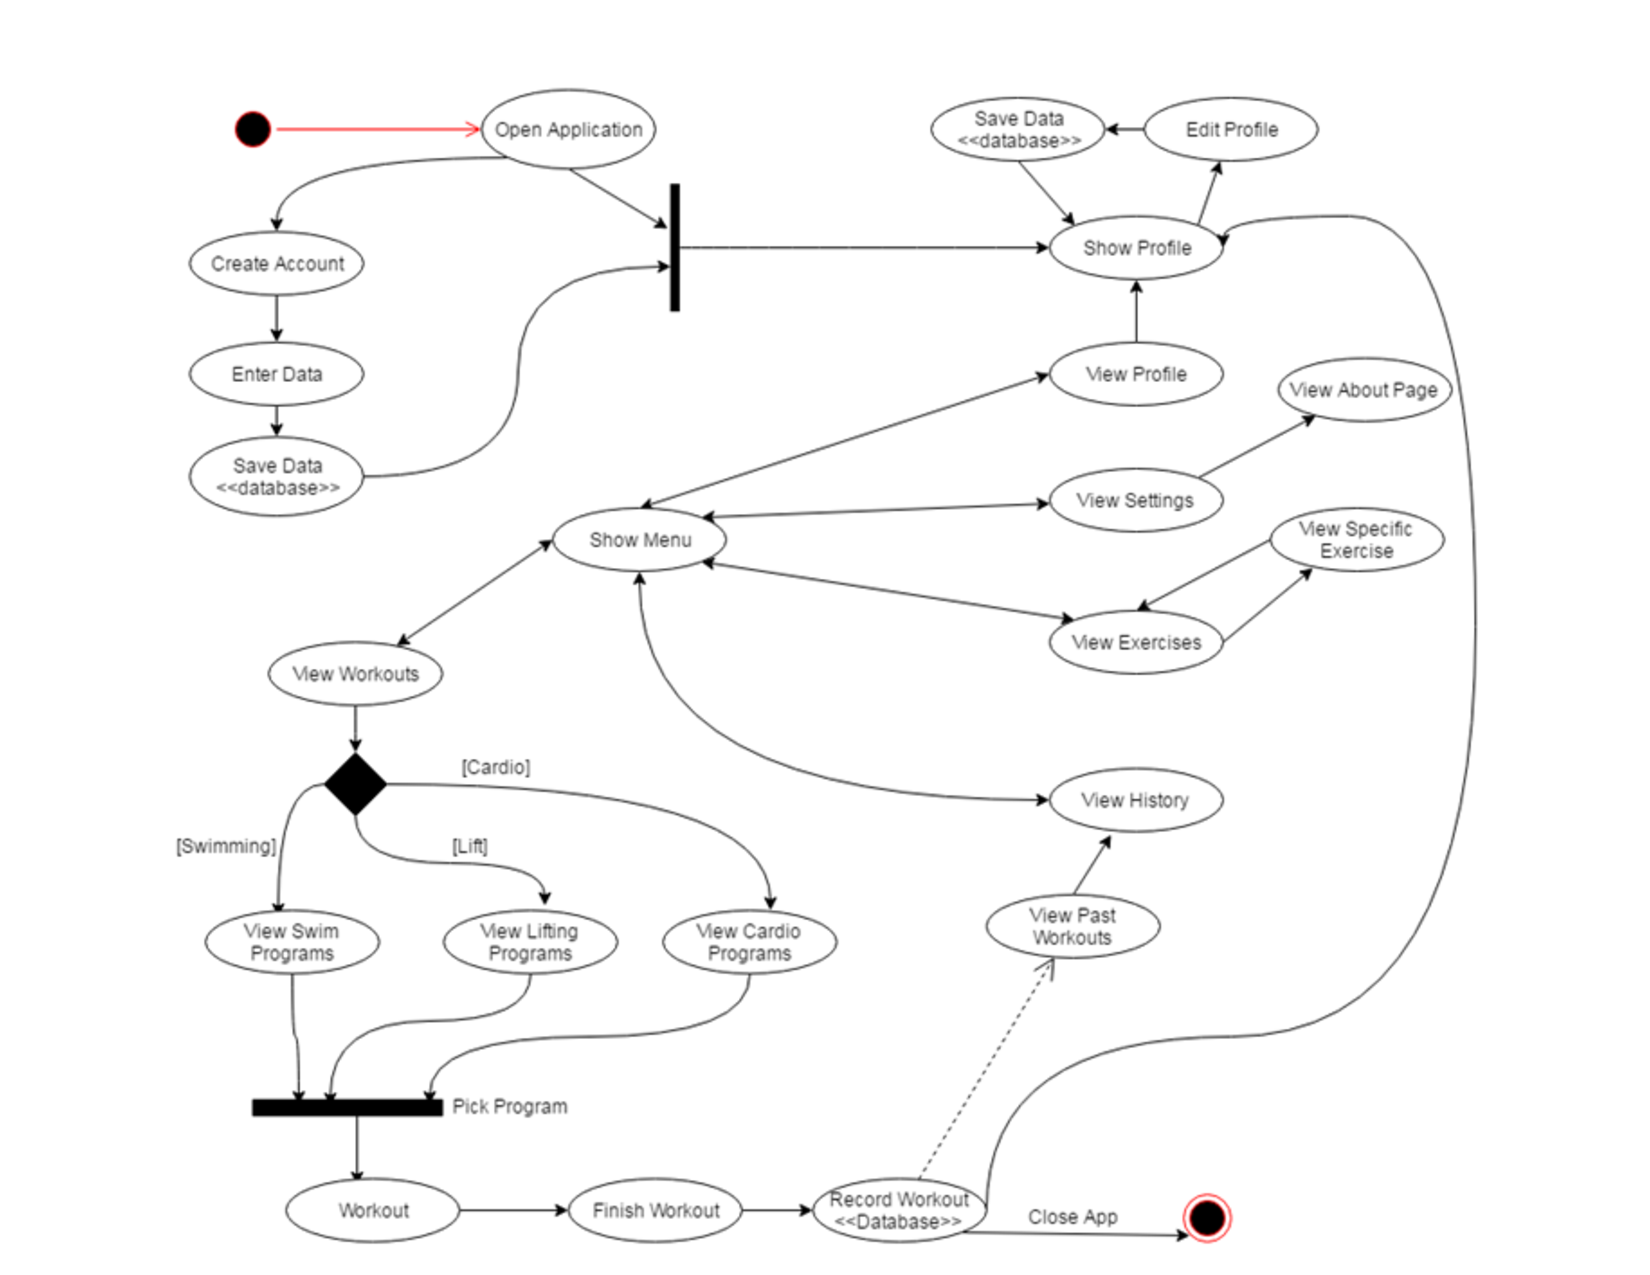
\includegraphics[width=5.0in]{./Figure/ativity.pdf}
\caption{Activity diagram of a system.}\label{fig:act_dia_1}
\end{figure*}

\subsection{Alternative Designs and Design Choices}
Describe alternative designs that were considered during execution of the project. Discuss how design choices were guided by constraints and other factors. E.g., architectural design models – Layered or Client-server and details shown using activity diagram as shown in Figure \ref{fig:act_dia_1} (Context model), sequence diagram (Interaction model), class diagram (Structural model).



\section{System Implementation}
This is the system inplementation section.

Describe the technical details for each of the subsystems or a the system-level and
provide sequence diagrams or station/activity diagrams for your system implemenation.



\section{System Testing}
This is the system testing section.

\subsection{Test Plan}
Provide your test plan with unit testing (Black-box testing and White-box testing), integration testing (Top-down or bottom-up approach) and system testing.

\subsection{Test Results}
Show your test restults and evaluate them. 

\section{Conclusions}
This is the conclusions section.

Overall summary of design methodologies, key creative approaches and potential
contribution/impact. \cite{hahahaha}

\bibliographystyle{IEEEtran}
\bibliography{Bibliography}


 
\end{document}